\documentclass[../Head/Main.tex]{subfiles}
\begin{document}
\section{Photogrammetry}\label{sec:photo}
In this section, the goal was to take the partially overlapping images taken by the drone, and stitch them together.\\
The aim is to get a large, high definition image, that looks like it was taken from a higher altitude, 
capturing a larger land area than any single original image from the set.\\
To create the orthomosaic, Agisoft Metashape Pro was chosen. 
Different quality settings where tried and results compared.

\subsection{EXIF data}
The images was taken 19\textsuperscript{th} of september 2017 from 10:01 AM to 10:41 AM. The footage was taken at Gyldensteen Gods at Gyldensteensvej 101, 5400 Bogense in an area contained by these four coordinates.
\begin{itemize}
\item[-] 55°33'59.99"N, 10°08'59.72"E \vspace{-7pt}
\item[-] 55°34'10.37"N, 10°08'59.72"E \vspace{-7pt}
\item[-] 55°34'10.37"N, 10°09'33.60"E \vspace{-7pt}
\item[-] 55°33'59.99"N, 10°09'33.60"E
\end{itemize}

The camera used was a senseFly S.O.D.A. with an image resolution of 5472 z 3648 pixels and a focal length of 10.2 mm/28 mm (35 mm equivalent). The type of UAV was not specified by the EXIF informations but it was either a senseFly eBee X or eBee Classic.\\
The images was taken on exposure priority with an exposure time of 1/1000 s and wide aperture of 2.8. The ISO-setting fluctuated from 200 to 800. The camera was set to auto white balance.

%Pitch                           : 6.029021
%Roll                            : -7.621159
%Yaw                             : 316.127563

\begin{figure}[H]
	\centering
	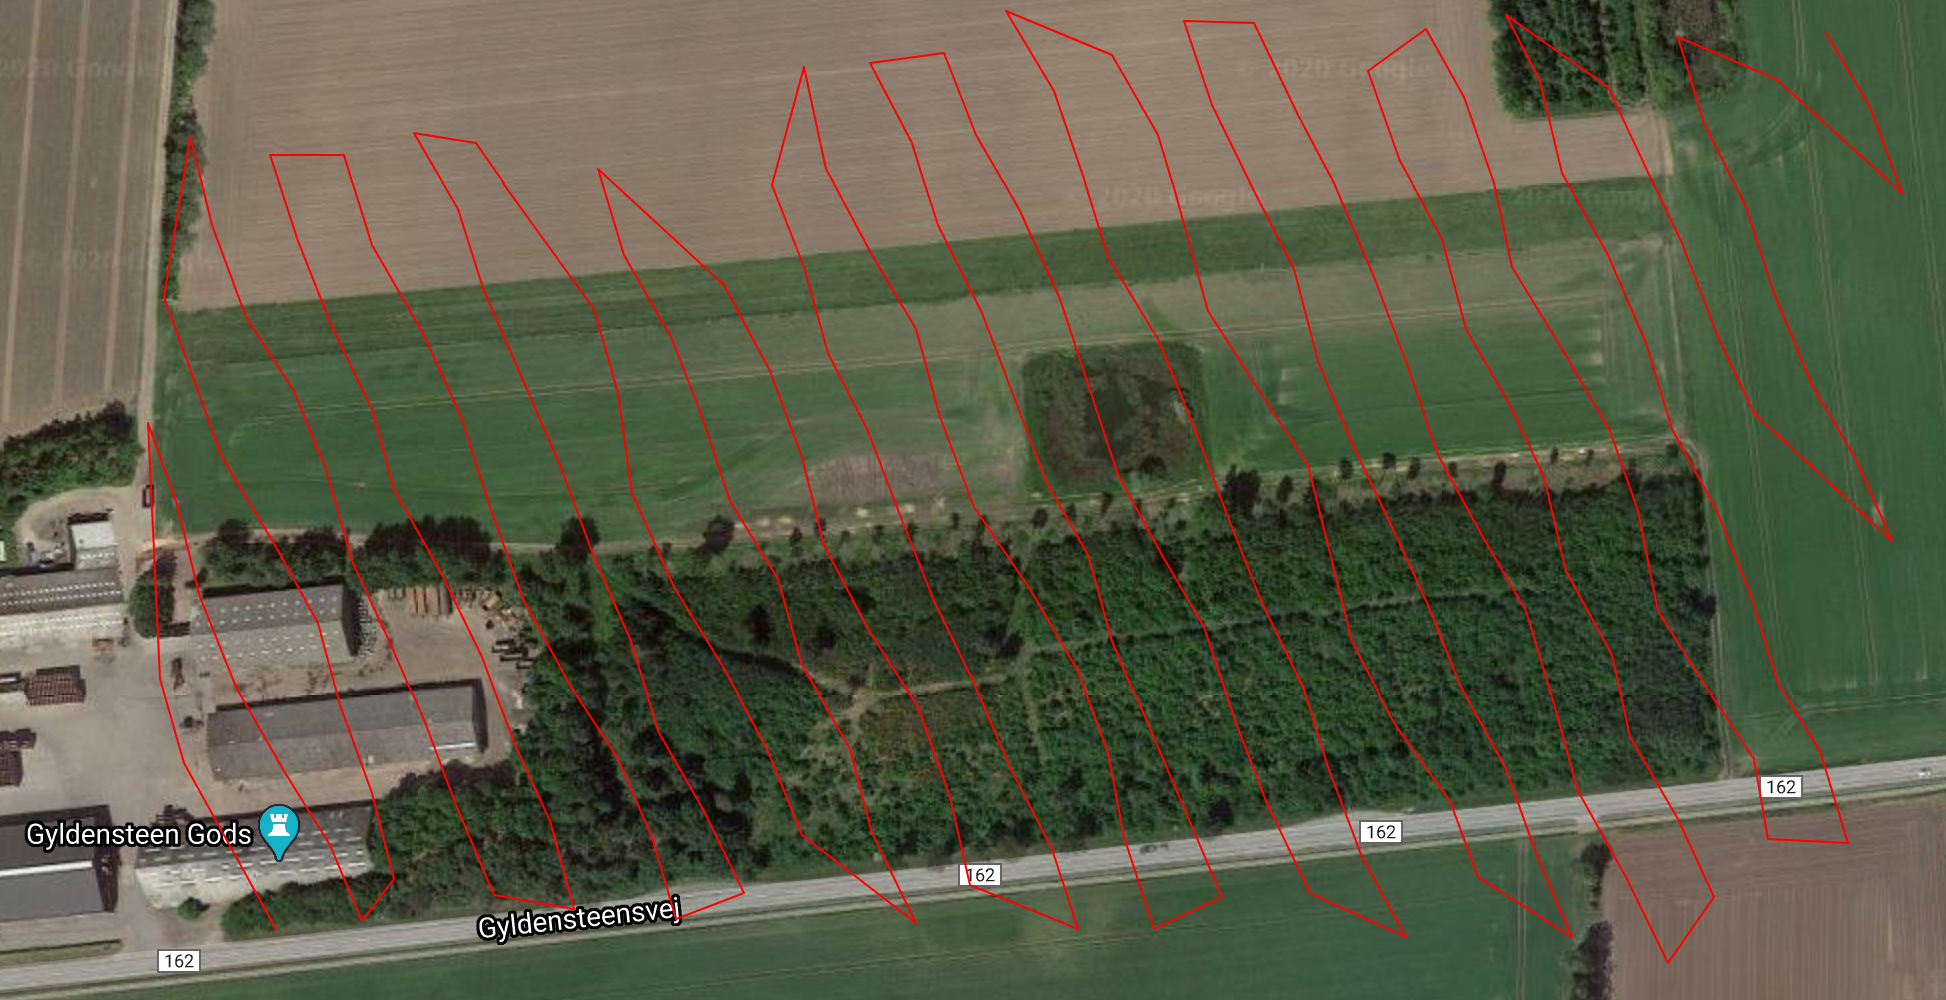
\includegraphics[width=0.75\textwidth]{../Figures/Flight_path}
	\caption{Illustration of the image path}
	\label{fig:flight_path}
	\vspace{-15pt}
\end{figure}
In figure \ref{fig:flight_path} the positions of the images taken can be seen. This is not the flight path of the drone, but the positions where the images where taken.

\subsection{Alignment}

The first step, after loading the images in Metashape, is to align them.
The alignment process looks for matching point pairs in multiple images and estimates their relative alignment based on the relative position offset of the point pairs.
We tried three quality options, medium, higher and highest.
The highest quality option failed, but both higher and medium ran successfully.
Both options took around a few seconds and there was no noticable difference in the results.

\subsection{Digital Elevation Model}
The digital elevation model is a 3D representation of a surface.
This can be computed by finding point pairs for each pixel and calculating from the disparity.
Not all pixels have pairs, in which case it can be estimated based on its neighbourhood.
For this computation, we left the parameters suggested by the program unchanged.

\subsection{Orthomosaic}
We tried different sources for the orthomosaic, in the end we chose to use the DEM.
For the final version, we left the parameters suggested by the program unchanged, except for the boundaries.
Since we only needed the field in the middle, we cut off the rest of the image through some trial and error.
The GSD resolution is 0.0235629 meters per pixel.

The largest file generated when exporting the orthomosaic was a 4 GB PNG, covering the whole image. 
The smallest file size we achieved, while still retaining good visual properties, was achieved with a 127 MB JPG with the unused parts cut off.
%IN THIS SECTION SHOULD BE INCLUDED:
%\begin{itemize}
%\item Bundle adjustment - check ✅✔
%\item Digitial elevation model - check ✅✔
%\item Orthorectification and orthomosaic creation - check
%\item EXIF data - check
%\item Number of images and approximate overlap
%\item Size of orthomosaic (resolution and disk size)
%\item Description of handling outside the fence data (cropping of the image)
%\item Screen shots of DSM and orthomosaic
%\end{itemize}
\end{document}